\section{Réalisation du projet}
Ce chapitre est l’occasion pour présenter les différents langage et outils utilisés pour réaliser le projet. Également, la mise en avant des différentes interfaces mises en œuvres pour l’exécution des différentes fonctionnalités. Enfin les tests effectués pour s’assurer du bon fonctionnement de logiciel.


\subsection {Langages \& outils utilisés}
\subsubsection {Langage R \& package Shiny}

\begin{figure}[!h]
	\center
	
\includegraphics[scale=0.2]{img/R_logo.png}
	\caption {Le logo du R project}
\end{figure}
R est un langage de programmation et un logiciel libre dédié aux statistiques et à la science des données soutenu par la R Foundation for Statistical Computing. Il est dérivé du langage S développé par John Chambers et ses collègues au sein des laboratoires Bell.\\
Le projet R naît en 1993 comme un projet de recherche de Ross Ihaka et Robert Gentleman à l'université d'Auckland (Nouvelle-Zélande). \\
Le langage R existe en plusieurs distribution, cependant la plus connue demeure celle du R Project et du Comprehensive R Archive Network (CRAN). Il existe d'autres distributions comme la distribution proposée par Microsoft14 ou encore celle de l'entreprise Oracle, Oracle R Distribution15.\\

\begin{figure}
	\center
	
\includegraphics[scale=0.3]{img/Shiny_logo.png}
	\caption {Le logo de Shiny}
\end{figure}
Shiny est un package R qui permet la création d'applications Web interactives directement à partir de R. Il permet d’héberger des applications autonomes sur une page Web ou les intégrer dans des documents R Markdown ou créer des tableaux de bord. Il offre également la possibilité d’étendre les applications Shiny avec des thèmes CSS, html widgets et des actions JavaScript, car le package entier repose sur ces différents langages. \\

Shiny permet de déployer une page web gérée par R et soutenu par HTML, CSS, Javascript et des framework reconnus comme Bootstrap ou encore Datatables.\\


R en combinaison avec Shiny ont étés adoptés en concertation avec nos encadrants et le maître d’ouvrage pour les raisons suivantes :
\begin{itemize} 
\item Les statistiques relatives aux classements des sportifs  devront être  faites en un langage capable de traiter des données volumineuses (les données relatives aux challenges dans le cas de notre projet) en réduisant au maximum les ressources utilisés en mémoire.
\item Des raisons pédagogiques. En fait, ce projet est l’occasion de découvrir les avantages et les limitations du langage R en termes de réalisation d’interfaces graphiques dynamiques et interactives.
\item La simplicité de développement : R est un langage dit de "Haut niveau", c'est à dire d'après Wikipédia : "un langage de programmation orienté autour du problème à résoudre, qui permet d'écrire des programmes en utilisant des mots usuels des langues naturelles (très souvent de l'anglais) et des symboles mathématiques familiers."
\item Un premier algorithme de classement a déjà été écrit, et fourni, en R.
\end{itemize}

Cependant, nous avons soulevé les point suivants :

\begin{itemize} 
	\item Déployer un serveur web fonctionnant sous R et Shiny n'est pas commun. Les hébergements web sont généralement en php.
	\item Les données concernés ne sont actuellement pas volumineuse, n'importe quel autre langage peut se permettre de les traiter avec autant d'efficacité.
	\item Shiny, avec l'appui des langages HTML, CSS et Javascript, se contente de générer une seule page web. Ce principe reste très réducteur de la fonction d'un site internet. De plus, cela oblige l'utilisateur à charger l'intégralité du site en une seule fois, incluant l'intégralité des données.
	\item Shiny permettant également de créer l'interface graphique, les étudiants ont émis des doutes quand à la création d'une interface graphique dynamique.
\end{itemize}

Pour le projet, les packages suivants ont également étés utilisés :

\begin{itemize} 
	\item "shinythemes", afin d'avoir une page web élégante.
	\item "DT", alias "DataTables", qui nous permet d'afficher des tableaux dynamiques avec énormément d'options intéressantes (Recherche, tri, mise en forme...)
	\item "xlsx", qui nous permet d'utiliser des fichiers Excel (Lire, enregistrer).
	\item "plyr", pour de la manipulation de tableaux avancée.
	\item "stats", pour des fonctions de statistique intéressante.
	\item "ggplot2", afin d'afficher des graphiques plus perfectionnés.
\end{itemize}

\newpage
\subsubsection {GitHub, LaTex, RStudio}

\begin{figure}[!h]
	\center
	
\includegraphics[scale=0.2]{img/desktop-logo.png}
	\caption {Le logo de GitHub}
\end{figure}
GitHub est un service web d'hébergement et de gestion de développement de logiciels, utilisant le logiciel de gestion de versions Git. \\
Le versionnage permet de travailler à plusieurs ur un code informatique, et de conserver l'historique des modifications du code. \\
GitHub propose ses services aux entreprises, mais le statut étudiant nous permet de privilégier d'un compte gratuit, nous permettant d'héberger notre code dans des répertoires privés.\\

\begin{figure}[!h]
	\center
	
\includegraphics[scale=0.1]{img/latex.png}
	\caption {Le logo de LaTex}
\end{figure}

LaTex est un langage et un système de composition de documents, qui nous a permis d'écrire ce rapport de manière efficace.

\begin{figure}[!h]
	\center
	
\includegraphics[scale=0.2]{img/rstudio.png}
	\caption {Le logo de LaTex}
\end{figure}

RStudio est un environnement de développement gratuit, libre et multiplateforme pour R.
L'ensemble des développements de ce projet ont étés effectués avec ce logiciel.


\newpage
\subsection {Les deux outils distincts du projet}
Pour permettre à l’utilisateur de bénéficier des fonctionnalités de notre logiciel, nous avons réalisé deux interfaces web. En effet, la première sera utilisée uniquement par l’administrateur de la ligue afin d’ajouter les différentes courses au challenge correspondant et également de consulter les informations et les statistiques relatives aux clubs et aux adhérents.

\subsubsection{Outil classement}

Dans un premier temps, l'outil "Classement" permet de réaliser les classements des sportifs. \\
Il s'agit uniquement d'un outil de calcul en ligne : l'utilisateur entre une course, un challenge (optionnel) et il pourra télécharger un classement mis à jour.

Voici trois aperçu de l'interface, pour chacun des onglets :

\begin{figure}[!h]
	\center
	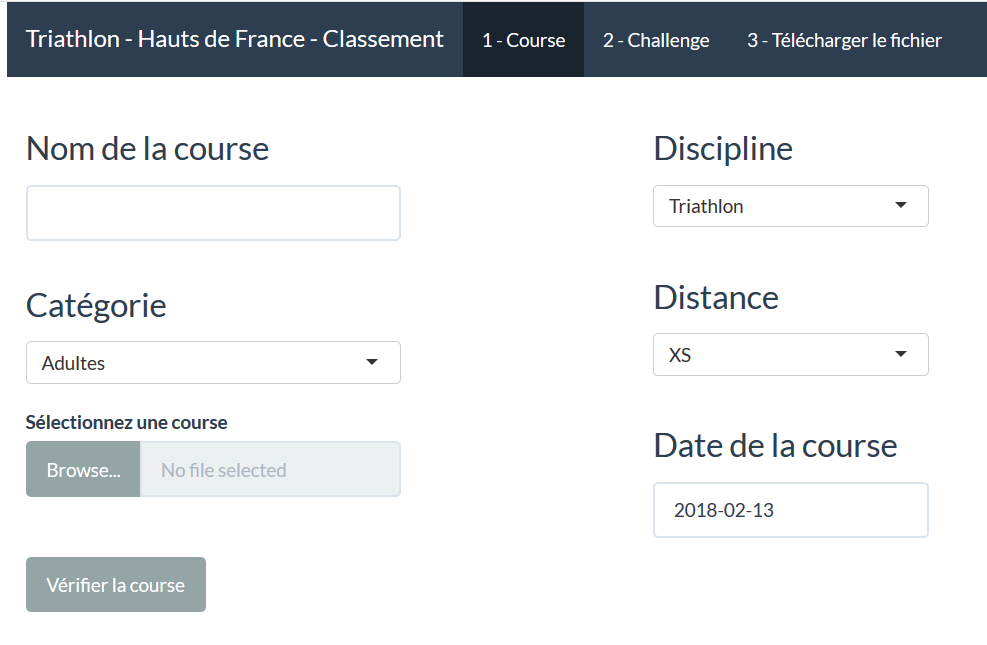
\includegraphics[scale=0.9]{img/admin_global.PNG}
	\caption {Aperçu de l'interface de classement - Onglet Course}
\end{figure}

\begin{figure}[!h]
	\center
	
\includegraphics[scale=0.9]{img/ex_challenge.PNG}
	\caption {Aperçu de l'interface de classement - Onglet Challenge}
\end{figure}

\begin{figure}[!h]
	\center
	
\includegraphics[scale=0.9]{img/ex_dl.PNG}
	\caption {Aperçu de l'interface de classement - Onglet Téléchargement}
\end{figure}

\newpage
Le processus se déroule en trois étapes :

\begin{enumerate} 
	\item La course à ajouter au challenge doit être vérifiée, l'administrateur doit donc entrer le fichier au format excel et certains paramètres :
	\begin{itemize} 
		\item Le nom de la course
		\item La discipline concernée (Triathlon, Duathlon, Aquathlon)
		\item La distance concernée (XS, S, M, L XL)
		\item La date de la course
		\item La catégorie (Adultes, Jeunes)
	\end{itemize}
	\item Le challenge existant peut être ajouté par l'administrateur, s'il ne l'est pas alors un nouveau challenge sera créé.
	\item Le challenge mis à jour est téléchargeable.
\end{enumerate}

Plus en détail, voici les différents points que l'algorithme aborde :

\begin{enumerate} 
	\item Gérer les erreurs de saisies utilisateur
	\item Vérifier la licence de l'utilisateur grâce au fichier Référence de la ligue.
	\item Gérer les éventuels cas d'Homonymes présents.
	\item Calculer les points gagnés pour la course.
	\item Intégrer le fichier course au fichier challenge, en vérifiant qu'une course du même nom n'existe pas.
	\item Calculer le classement par club.
	\item Enregistrer le fichier et le télécharger.
\end{enumerate}

Pour rappel, un code R nous a été fourni qui calculait ces classements. Nous avons travaillé dessus, puis remis à jour.
Voici un exemple de ce qu'il est possible de faire grâce à l'interprétation matricielle de R, en évitant d'utiliser des boucles.
Un aperçu ci-dessous du classement par clubs, original puis retravaillé à l'aide des fonctionnalités de R :

\begin{figure}[!h]
	\center
	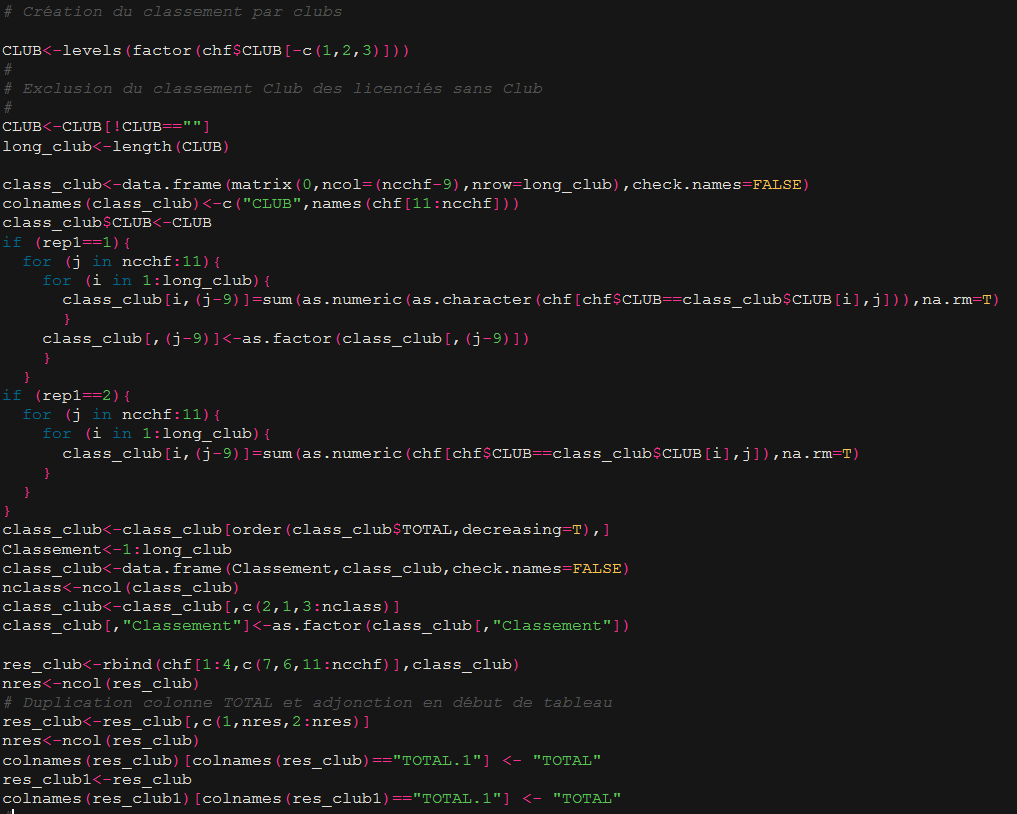
\includegraphics[scale=0.9]{img/codeoriginal.PNG}
	\caption {Code du classement par clubs - Original}
\end{figure}

\begin{figure}[!h]
	\center
	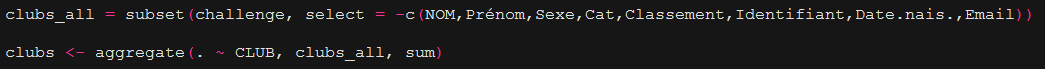
\includegraphics[scale=0.9]{img/codenew.PNG}
	\caption {Code du classement par clubs - Nouveau}
\end{figure}


\subsubsection{Outil challenge}

Dans un second temps, l'outils "Challenge" permet d'afficher ces résultats dans un format intéressant.
Dans une seule page web seront contenu tout les tableaux de résultats des différentes années à partir de 2017, et ce pour les catégories Adultes et Jeunes, ainsi que pour les Clubs.

Voici un aperçu de l'interface web :

\begin{figure}[!h]
	\center
	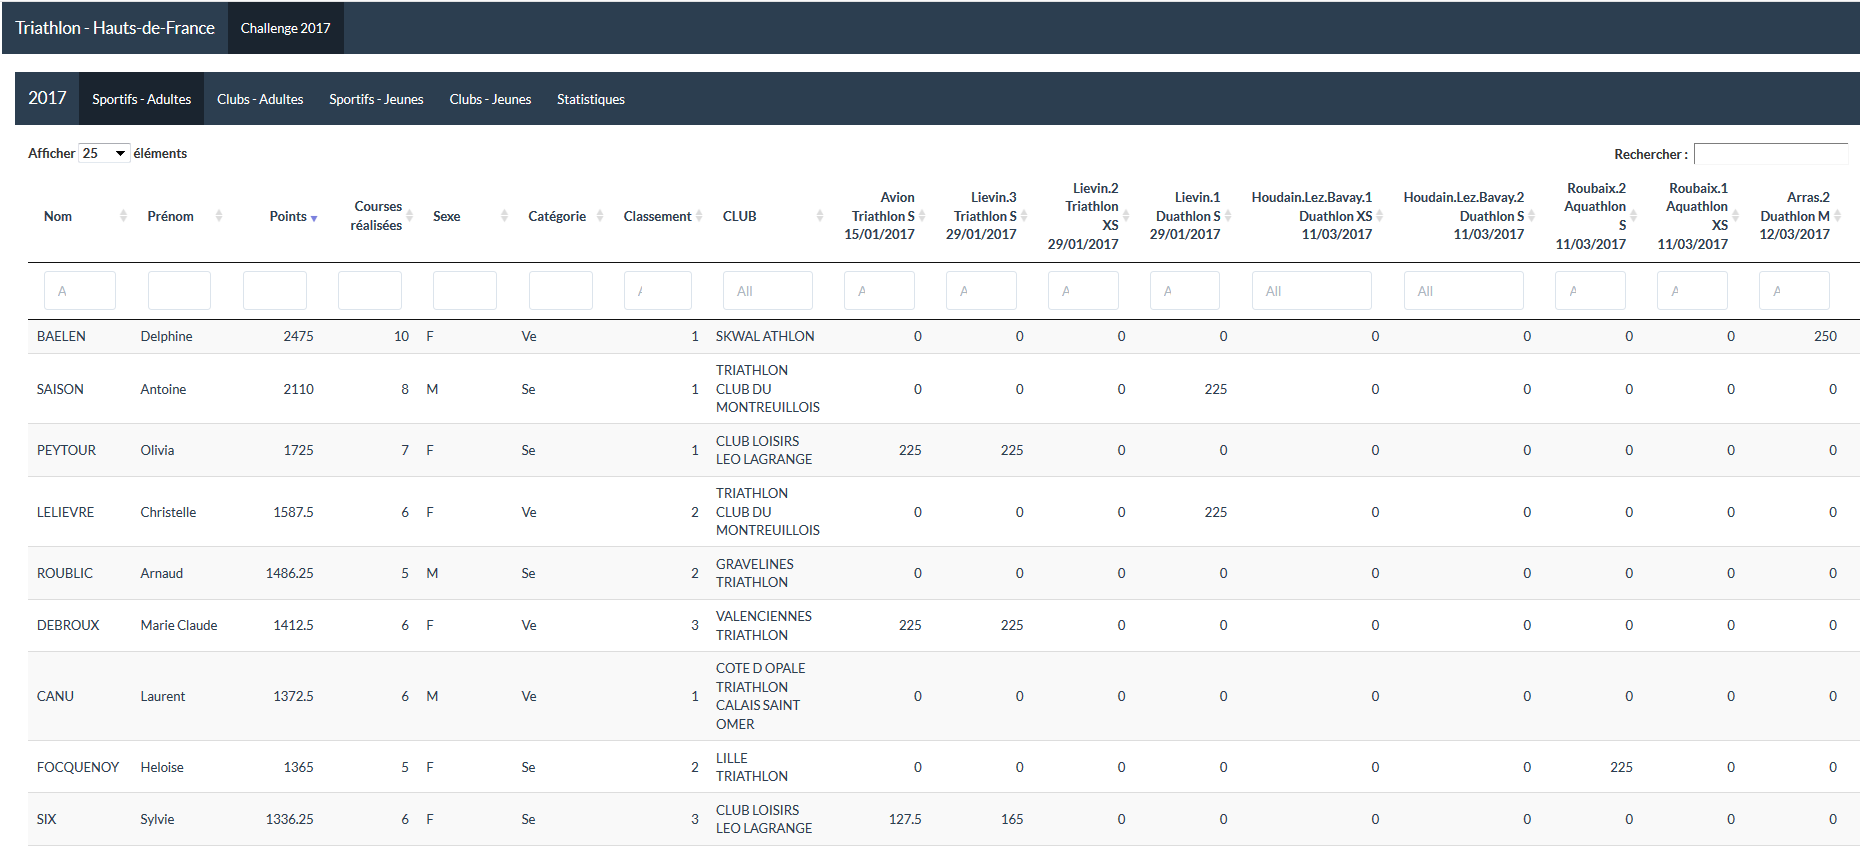
\includegraphics[scale=0.45]{img/online.PNG}
	\caption {Aperçu de l'interface web affichant les résultats}
\end{figure}

Voici les éléments composant cette interface :

\begin{itemize} 
	\item Une barre d'onglet pour les années du challenge, pour le moment uniquement 2017.
	\item Une barre d'onglet pour l'année courante, comportant les challenge adultes et jeunes ainsi que les classements par clubs.
	\item Le tableau de résultat.
\end{itemize}

Les avantages offert par le plugin DataTables sont :

\begin{itemize} 
	\item Une recherche globale, en haut à droite du tableau.
	\item Un tri possible pour toute les colonnes.
	\item Une recherche possible pour toute les colonnes.
	\item La sélection de lignes.
	\item Un affichage dynamique sur plusieurs pages.
\end{itemize}

En cliquant sur la ligne d'un participant, des statistiques plus précise sont disponible ainsi que ses informations personnelles.
Ainsi, un indice de performance est calculé, globalement, par sexe et enfin par catégorie. \\

Des statistiques globales sont également présentes, dans l'onglet correspondant.
En voici un aperçu :


\begin{figure}[!h]
	\center
	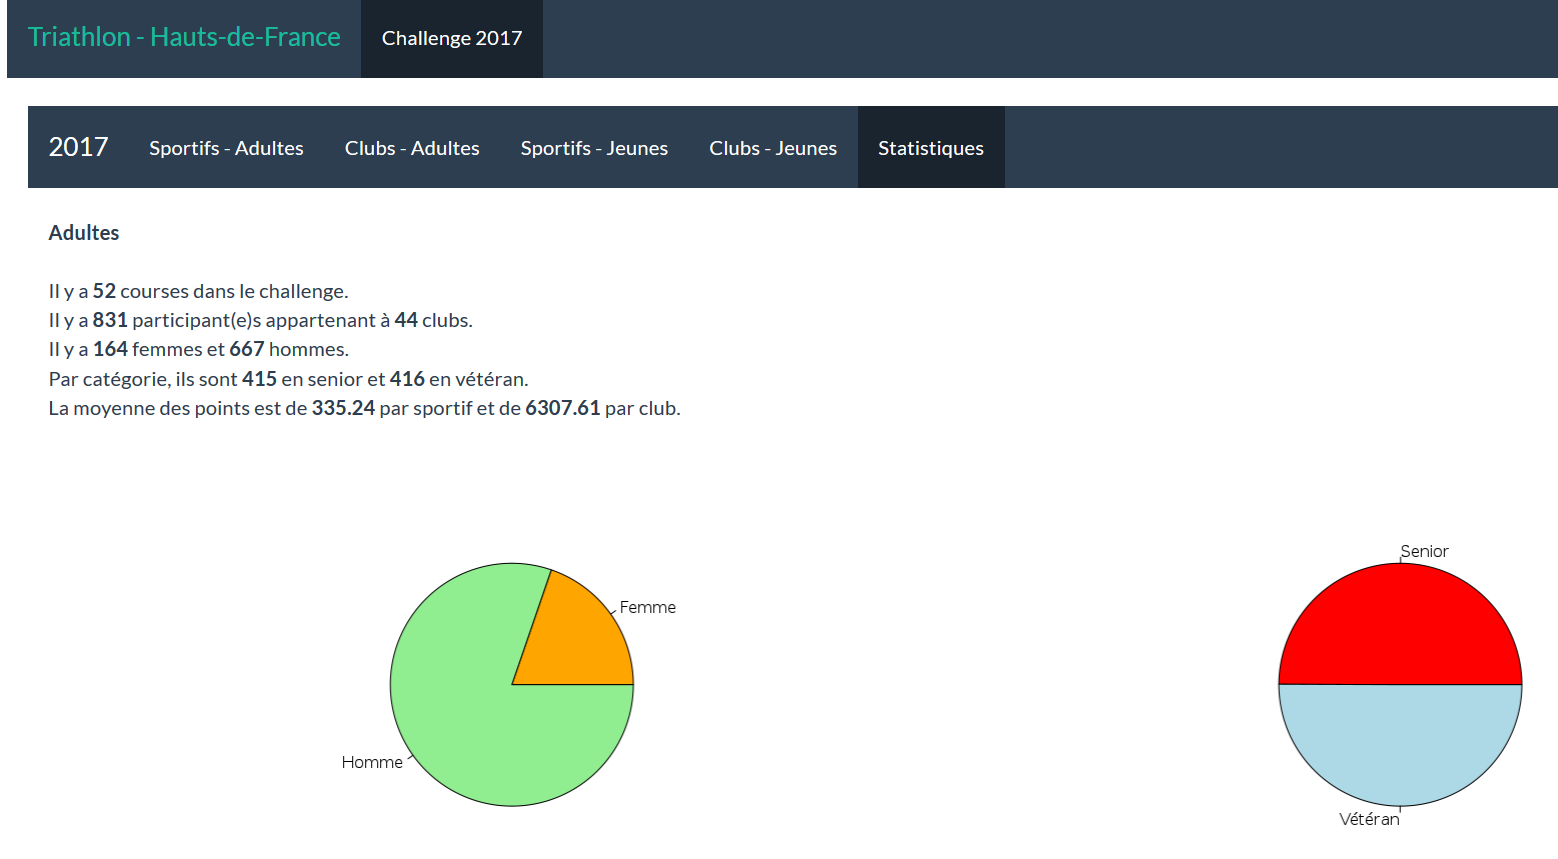
\includegraphics[scale=0.55]{img/statsad.PNG}
	\caption {Statistiques globales adultes}
\end{figure}
\begin{figure}[!h]
	\center
	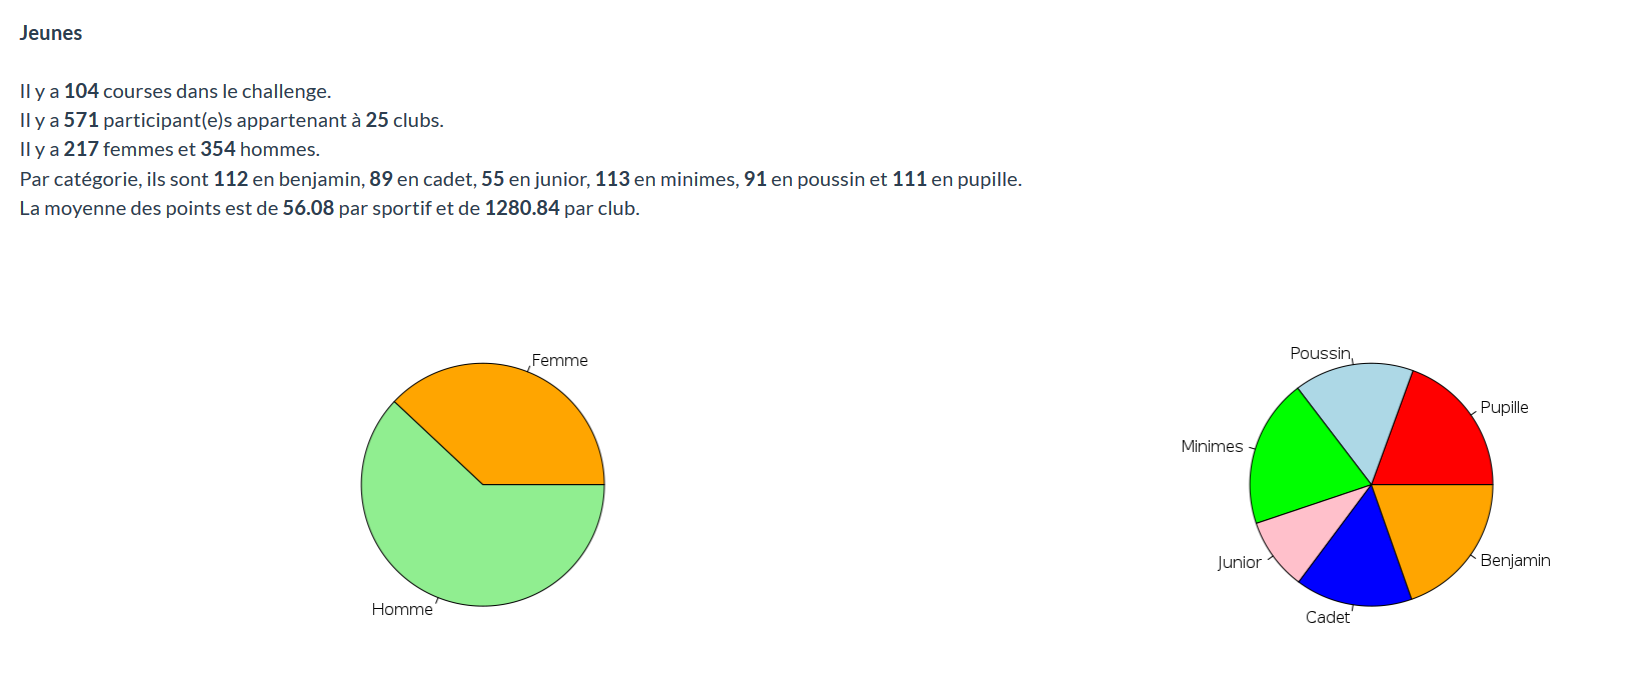
\includegraphics[scale=0.55]{img/statsjn.PNG}
	\caption {Statistiques globales jeunes}
\end{figure}


\subsection {Déploiement du projet}

Comme énoncé précédemment, le projet a besoin d'un serveur R shiny pour déployer les outils sur le web.
Pour cela nous disposons d'un serveur personnel debian ainsi que d'une adresse ipv4 valide.

Voici comment s'est déroulé ce déploiement :

\begin{enumerate} 
	\item Installation de R, avec les packages nécessaires cités pus haut. \cite{ref2}
	\item Installation de shiny-server \cite{ref3}
	\item Configuration de shiny-server : deux serveurs lancés, l'un sur le port 3838 et l'autre sur le 3939. Les deux pointent vers deux dossiers de l'utilisateur "triathlon" créé pour l'occasion.
	\item Grâce aux identifiants OVH \cite{ref4} fournis par la ligue, nous avons eu accès au nom de domaine "triathlonhdf.fr" (où leur nouveau site web venait d'être déployé) et avons créés les sous-domaine challenge.triathlonhdf.fr et classement.triathlonhdf.fr. Ces deux sous-domaines pointent à l'aide d'une redirection invisible vers notre ipv4 et le port souhaité.
	\item Un accès FTP sera fourni à la ligue afin de modifier les fichiers excel nécessaire au fonctionnement.
\end{enumerate}


\subsection {La documentation automatique}
La documentation du projet consiste commenter toutes les fonctions pour faciliter la compréhension du codes et les changements futurs à effectuer.
Dans le cadre de notre projet,  la documentation  consiste à ajouter les commentaires concernant les boucles et les conditions utilisées au sein du code.


\subsection {Schéma des tests}
Les tests revêtent une importance capitale avant, lors et après le déploiement du logiciel sur le serveur. En effet, ils permettent d'identifier un nombre maximum de comportements problématiques du logiciel afin d'en augmenter la qualité.Ainsi, il demeure important de  le schéma et le type de tests à effectuer. \\
Dans cette optique, nous avons décider d'effectuer des tests unitaires pour chaque fonctionnalité implémentée, un test global pour l'ensemble du projet et à la fin un test d'acceptation lors du déploiement du projet sur le serveur dédié.\\
L'ensemble de ces tests concernent les deux modules développés à savoir :
-l'outil de classement; 
-l'outil challenge.

\subsubsection{Outil classement}
La première phase  des tests sur l'outil challenge consiste en la validation du code  Comparaison.R fourni et Challenge.R . Par conséquent, les tests effectués sont répertoriés comme suit :
\begin{itemize}
\item Tester les la modification des entêtes du fichiers Excel
\item Tester le choix des valeurs qui doivent être entrées par l'utilisateurs
\item Tester l'existence du fichier xl de la course
\item Tester l'existences des homonymes(validé)
\item Tester  l'ajout d'une course
\item Tester les homonymes
\end{itemize}
\subsubsection{Outil challenge}

S'agissant de l'outil challenge, les tests réalisé sont les suivants:
\begin{itemize}
\item La visualisation des résultats sous la forme dans un tableau sur l'interface graphique
\item Tester le tri des résultats sur tous les critères spécifiés par le  client (tri selon le sexe, la catégorie, ...)
\item La visualisation des résultats d'un seul sportif en cliquant sur la ligne correspondante
\item L'affichage des graphes représentant les statistiques à chaque sportif.
\end{itemize}
 
Dans cette optique, nous avons décider d'effectuer des tests unitaires pour chaque fonctionnalité implémentée, un test global pour l'ensemble du projet et à la fin un test d'acceptation lors du déploiement du projet sur le serveur dédié.\\

Dans cette optique, nous avons décider d'effectuer des tests unitaires pour chaque fonctionnalité implémentée, un test global pour l'ensemble du projet et à la fin un test d'acceptance lors du déploiement du projet sur le serveur dédié.\\

S'agissant de l'outil challenge, les tests réalisé sont les suivants:
\begin{itemize}
\item La visualisation des résultats sous la forme dans un tableau sur l'interface graphique
\item Tester le tri des résultats sur tous les critères spécifiés par le  client (tri selon le sexe, la catégorie, ...)
\item La visualisation des résultats d'un seul sportif en cliquant sur la ligne correspondante
\item L'affichage des graphes représentant les statistiques de chaque sportif.
\end{itemize}


                                                                                                                                                                                                                                                ensemble de ces tests concernent les deux modules développés à savoir :


